\section{Simulation Analysis}
\label{sec:simulation}
In this section we will describe the steps needed to simulate this circuit using the software Ngspice.
\subsection{Operating Point Analysis}
\textbf{Table~\ref{tab:op}} shows the simulated operating point results for the circuit
under analysis. The current flows considered in the theoretical section were coherent with the polarity implicitly declared when defining the circuit to be simulated in the Ngspice script.\par
As mentioned previously, in Section~\ref{sec:analysis}, we had to create a "fictional" voltage source, between node 7 and resistor 6 (providing 0V to the circuit in order not to alter the behaviour of the rest of the circuit) so as to be able to define the dependecy for the current-controlled voltage source {\it $V_c$}. This has no specific reason to be, other than the particularities of the Ngspice software. The consequences of adding this additional voltage have already been described (namely the creation of a new node) and dealt with in the previous section - see, for example, equation \ref{eq:n2}.\par
The following steps in the simulations are to be conducted: 
\begin{itemize}
	\item for t<0 (operating point only, in order to obtain the voltages in all nodes and the currents in all branches);
	\item operating point for {\it $V_s(0) = 0$}, replacing the capacitor with a a voltage source Vx = V(6)-V(8), where V(6) and V(8) are the voltages in nodes 6 and 8 as obtained in the previous step (this step is necessary given that we must the compute the boundary conditions that guarantee continuity in the capacitor's discharge - such may imply that the boundary conditions differ from those computed for t<0);
	\item for the natural response of the circuit (using the boundary conditions V(6) and V(8) as obtained previously);
	\item repeating the third step, for the natural and forced response on node 6 with {\it $V_s$} (as given in \textbf{Figure~\ref{fig:time_step}}) and f = 1kHz.
	\item for the frequency response in node 6 given these conditions
\end{itemize}

\begin{figure}[h] \centering
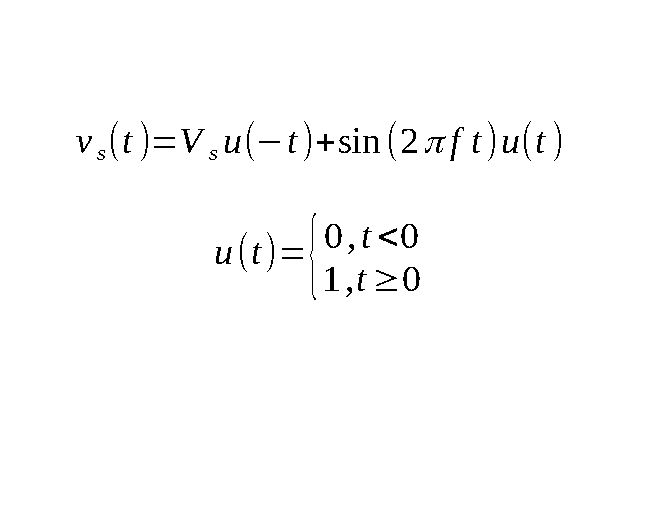
\includegraphics[width=0.5\linewidth]{time_step.pdf}
\caption{Time step conditions}
\label{fig:time_step}
\end{figure}

\begin{table}[h]
  \centering
  \begin{tabular}{|l|r|}
    \hline    
    {\bf Name} & {\bf Value [mA or V]} \\ \hline
    @c[i] & 0.000000e+00\\ \hline
@gb[i] & -2.91567e-04\\ \hline
@r1[i] & 2.780494e-04\\ \hline
@r2[i] & 2.915672e-04\\ \hline
@r3[i] & -1.35178e-05\\ \hline
@r4[i] & -1.22689e-03\\ \hline
@r5[i] & -2.91567e-04\\ \hline
@r6[i] & 9.488377e-04\\ \hline
@r7[i] & 9.488377e-04\\ \hline
v(1) & 5.243596e+00\\ \hline
v(2) & 4.952739e+00\\ \hline
v(3) & 4.367468e+00\\ \hline
v(4) & -1.96340e+00\\ \hline
v(5) & 4.994112e+00\\ \hline
v(6) & 5.904536e+00\\ \hline
v(7) & -1.96340e+00\\ \hline
v(8) & -2.92677e+00\\ \hline

  \end{tabular}
  \caption{Operating point. A variable preceded by @ is of type {\em current}
    and expressed in miliAmpere; other variables are of type {\it voltage} and expressed in
    Volt.}
  \label{tab:op}
\end{table}

As can already be observed, the results of the simulation coincide up to the last digit with the results of the theoretical analysis.
